% Fintech Multi-Agent Orchestrator -- Technical Guide
\documentclass[12pt,a4paper]{article}

\usepackage[margin=2.8cm]{geometry}
\usepackage{listings}
\usepackage{tikz}
\usepackage{booktabs}
\usepackage{parskip}
\usepackage{float}
\usepackage{hyperref}
\usepackage{caption}

\usetikzlibrary{arrows.meta, positioning}

\lstset{
  basicstyle=\ttfamily\footnotesize,
  breaklines=true,
  frame=single,
  numbers=left,
  numberstyle=\tiny,
  numbersep=8pt,
  tabsize=2,
  showstringspaces=false,
  language=Python
}

\hypersetup{hidelinks}
\captionsetup{font=small, labelfont=bf}

\title{\textbf{Fintech Multi-Agent Orchestrator}\\[0.4em]
       \large A Technical Guide}
\author{}
\date{}

% ------------------------------------------------------------------
% Helper: a table wrapped in a float with a caption
% Usage: wrap tabular environments in \begin{table}[H]\centering...\end{table}
% ------------------------------------------------------------------

\begin{document}

\maketitle
\tableofcontents
\newpage


% ==================================================================
\section{What Is This System?}
% ==================================================================

This is a question-answering system for a finance operations team. An analyst types a question like:

\begin{quote}
\textit{``Which funds have breached their risk limits today, and what does the mandate say about the cash minimum?''}
\end{quote}

The system figures out what the question is asking for, fetches the relevant data, runs the appropriate analysis, checks its own answer for quality, and returns a formatted report.

The key idea is \textbf{orchestration}. A single AI model call cannot reliably do all of this. Instead, the system breaks the work into steps and runs a chain of specialised components -- each responsible for one part -- passing results forward until the job is done.

\subsection{The analogy}

Think of a small internal consulting team. A client brief arrives. A project manager reads it and assigns it. A data analyst pulls the numbers. A risk analyst checks them against compliance rules. A report writer assembles the findings. A reviewer approves the draft before it goes out.

This system automates exactly that workflow. Each role is replaced by a software component backed by an AI model.

\subsection{Key vocabulary}

The following terms are used throughout this document.

\begin{table}[H]
\centering
\small
\begin{tabular}{@{}p{3.2cm}p{10.5cm}@{}}
\toprule
\textbf{Term} & \textbf{Meaning} \\
\midrule
LLM & Large Language Model. The AI that generates text -- Claude, GPT-4, etc. Think of it as a function: text goes in, text comes out. \\
\addlinespace
Agent & A module that uses an LLM for one specific job. Each agent has a system prompt that defines its role. \\
\addlinespace
Tool & A regular Python function the LLM is allowed to call. The LLM requests ``run this SQL query''; the tool executes it and returns the result. \\
\addlinespace
Structured output & Forcing the LLM to return a specific JSON shape instead of free text. The shape is validated against a Pydantic model. \\
\addlinespace
State machine & A program that moves through a fixed set of phases (supervising, executing, validating, ...) via defined transitions. \\
\bottomrule
\end{tabular}
\caption{Vocabulary used in this document}
\end{table}


% ==================================================================
\section{Technology Choices}
% ==================================================================

\begin{table}[H]
\centering
\small
\begin{tabular}{@{}p{2.4cm}p{4.8cm}p{6.5cm}@{}}
\toprule
\textbf{Library} & \textbf{Role} & \textbf{Key reason for choosing it} \\
\midrule
LangGraph   & Orchestrates the workflow          & Built specifically for multi-step LLM pipelines \\
LangChain   & LLM and tool interface             & Abstracts provider differences (Claude vs GPT) \\
FastAPI     & HTTP API                           & Async-native; generates docs automatically \\
Pydantic    & Data modelling and validation      & Catches bad data at runtime with clear errors \\
Redis       & Task state and audit storage       & Fast, async, supports TTL and sorted sets \\
SQLite      & Placeholder database               & Zero setup; swap for a real DWH in production \\
ChromaDB    & Document search                    & Runs in-process; no extra service needed \\
Claude      & LLM provider                       & Strong structured output; 200k token context \\
slowapi     & Rate limiting                      & One decorator per route \\
structlog   & Logging                            & Outputs structured JSON \\
\bottomrule
\end{tabular}
\caption{Full technology stack}
\end{table}

\subsection{Why Python?}

The LangChain and LangGraph ecosystems are Python-first. The entire industry converged on Python for LLM work. Using another language would mean reimplementing these libraries from scratch.

\subsection{Why async throughout?}

LLM API calls take 2--20 seconds. A blocking server could handle only one request at a time. Python's \texttt{asyncio} lets a single process handle many in-flight requests concurrently. FastAPI, LangGraph, Redis, and the database clients are all async-native.


% ==================================================================
\section{Architecture}
% ==================================================================

The system has four layers, each with a single clear responsibility.

\begin{figure}[H]
\centering
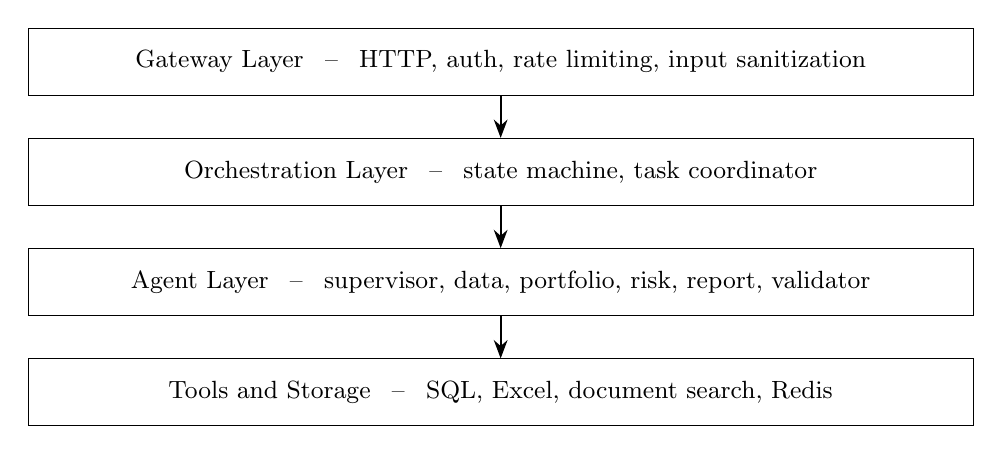
\begin{tikzpicture}[
  box/.style={draw, rectangle, minimum width=12cm, minimum height=0.85cm,
              text centered, font=\small},
  arr/.style={-Stealth, thick}
]
  \node[box] (g) at (0, 0)    {Gateway Layer \enspace -- \enspace HTTP, auth, rate limiting, input sanitization};
  \node[box] (o) at (0,-1.4)  {Orchestration Layer \enspace -- \enspace state machine, task coordinator};
  \node[box] (a) at (0,-2.8)  {Agent Layer \enspace -- \enspace supervisor, data, portfolio, risk, report, validator};
  \node[box] (t) at (0,-4.2)  {Tools and Storage \enspace -- \enspace SQL, Excel, document search, Redis};
  \draw[arr] (g.south) -- (o.north);
  \draw[arr] (o.south) -- (a.north);
  \draw[arr] (a.south) -- (t.north);
\end{tikzpicture}
\caption{Four-layer architecture. Dependencies only flow downward.}
\end{figure}

The important constraint is that dependencies only flow downward. The agent layer imports from the tools layer, but the tools layer never imports from agents. This means each layer can be tested in isolation.


% ==================================================================
\section{How a Request Flows}
% ==================================================================

\begin{figure}[H]
\centering
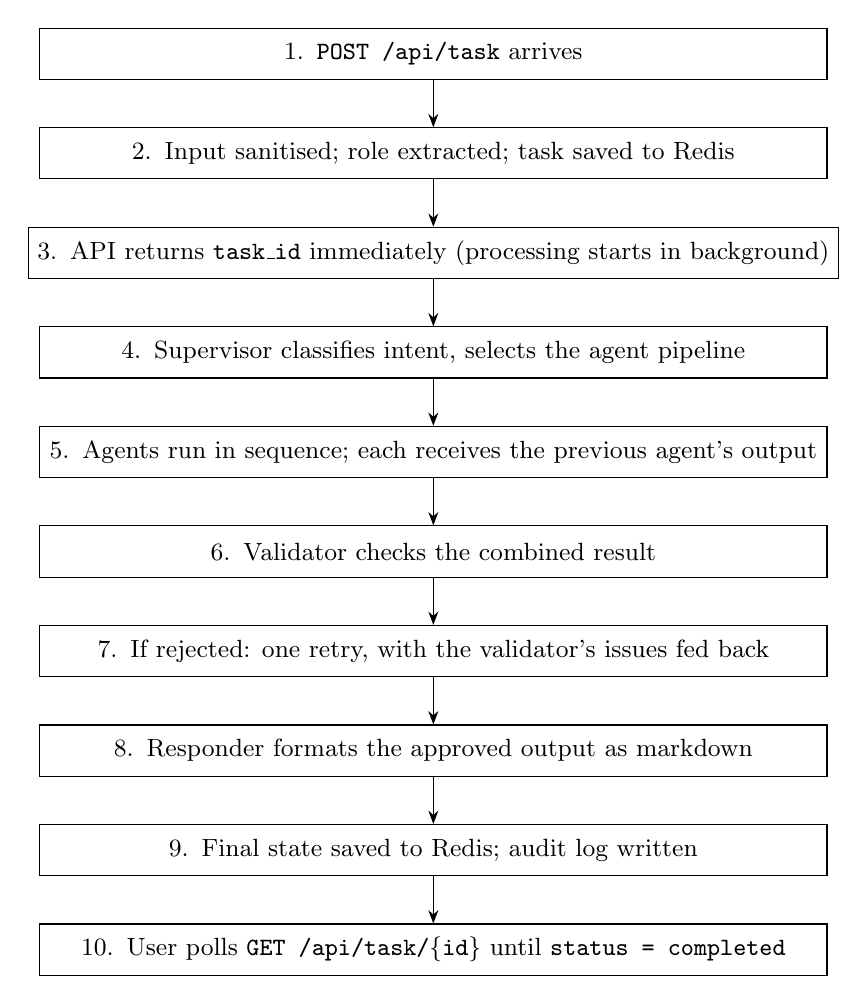
\begin{tikzpicture}[
  node distance=0.6cm,
  box/.style={draw, rectangle, minimum width=10cm, minimum height=0.65cm,
              text centered, font=\small},
  arr/.style={-Stealth}
]
  \node[box] (a) {1.\enspace \texttt{POST /api/task} arrives};
  \node[box, below=of a] (b) {2.\enspace Input sanitised; role extracted; task saved to Redis};
  \node[box, below=of b] (c) {3.\enspace API returns \texttt{task\_id} immediately (processing starts in background)};
  \node[box, below=of c] (d) {4.\enspace Supervisor classifies intent, selects the agent pipeline};
  \node[box, below=of d] (e) {5.\enspace Agents run in sequence; each receives the previous agent's output};
  \node[box, below=of e] (f) {6.\enspace Validator checks the combined result};
  \node[box, below=of f] (g) {7.\enspace If rejected: one retry, with the validator's issues fed back};
  \node[box, below=of g] (h) {8.\enspace Responder formats the approved output as markdown};
  \node[box, below=of h] (i) {9.\enspace Final state saved to Redis; audit log written};
  \node[box, below=of i] (j) {10.\enspace User polls \texttt{GET /api/task/\{id\}} until \texttt{status = completed}};
  \foreach \x/\y in {a/b, b/c, c/d, d/e, e/f, f/g, g/h, h/i, i/j}
    \draw[arr] (\x.south) -- (\y.north);
\end{tikzpicture}
\caption{End-to-end request lifecycle}
\end{figure}

Step 3 is the key design point: the API returns immediately. The actual LLM processing happens in a background async task. This means the HTTP connection does not stay open while the model works.

The user polls step 10 until the status changes. This is called the \textbf{polling pattern} and is common for background jobs that take more than a few seconds.


% ==================================================================
\section{The Orchestration Graph}
% ==================================================================

\subsection{What LangGraph does}

LangGraph is a library for writing workflows as directed graphs. Each \textbf{node} is an async Python function. Each \textbf{edge} says which node runs next. Some edges are \textbf{conditional} -- the next node depends on a value in the current state.

The entire state of a task lives in a single Python dictionary called \texttt{OrchestratorState}. Every node receives this dictionary and returns an updated copy. Nothing is stored globally.

\subsection{The graph structure}

\begin{figure}[H]
\centering
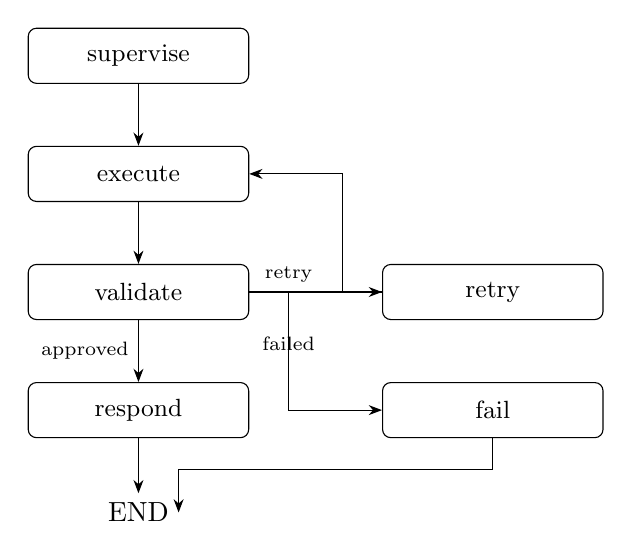
\begin{tikzpicture}[
  n/.style={draw, rectangle, rounded corners=3pt, minimum width=2.8cm, minimum height=0.7cm,
            text centered, font=\small},
  arr/.style={-Stealth}
]
  \node[n] (s)  at (0, 0)    {supervise};
  \node[n] (e)  at (0,-1.5)  {execute};
  \node[n] (v)  at (0,-3.0)  {validate};
  \node[n] (r)  at (0,-4.5)  {respond};
  \node[n] (rt) at (4.5,-3.0){retry};
  \node[n] (f)  at (4.5,-4.5){fail};
  \node[draw=none] (end) at (0,-5.8) {END};

  \draw[arr] (s) -- (e);
  \draw[arr] (e) -- (v);
  \draw[arr] (v) -- node[left, font=\scriptsize]{approved} (r);
  \draw[arr] (v.east) -- ++(0.5,0) |- node[above, font=\scriptsize, pos=0.25]{retry} (rt.west);
  \draw[arr] (v.east) -- ++(0.5,0) |- node[below, font=\scriptsize, pos=0.15]{failed} (f.west);
  \draw[arr] (rt.west) -- ++(-0.5,0) |- (e.east);
  \draw[arr] (r.south) -- (end.north);
  \draw[arr] (f.south) -- ++(0,-0.4) -| (end.east);
\end{tikzpicture}
\caption{Graph nodes and transitions. The retry node loops back into execute.}
\end{figure}

\begin{table}[H]
\centering
\small
\begin{tabular}{@{}p{2.2cm}p{11.5cm}@{}}
\toprule
\textbf{Node} & \textbf{What it does} \\
\midrule
supervise & Classifies the user's intent and selects the list of agents to run. \\
execute   & Runs each agent in sequence, passing each agent's output to the next. \\
validate  & Checks the combined output for completeness, accuracy, and safety. \\
retry     & Increments the retry counter and routes back to execute. Allowed once. \\
respond   & Formats the approved output into a final markdown response. \\
fail      & Handles the case where validation keeps rejecting or the budget is exceeded. \\
\bottomrule
\end{tabular}
\caption{What each graph node does}
\end{table}

\subsection{The task state}

Every node reads from and writes to the same object. The fields below are the most important ones.

\begin{lstlisting}[caption={Core fields of OrchestratorState}]
class OrchestratorState(TypedDict):
    task_id: str
    user_id: str
    task: str              # the user's original question

    intent: str            # e.g. "risk_report" -- set by supervise
    agents_selected: list  # e.g. ["data", "risk", "report"]
    agent_results: dict    # agent_name -> {status, result}

    validation_result: ValidationResult
    retry_count: int

    final_response: str    # the markdown answer returned to the user
    cost_tracking: CostTracking
\end{lstlisting}

Because all state is in one place, debugging is straightforward: print the state at any node and you can see exactly where things stand.


% ==================================================================
\section{The Agent Layer}
% ==================================================================

\subsection{Overview of all agents}

\begin{table}[H]
\centering
\small
\begin{tabular}{@{}p{3.2cm}p{3.2cm}p{7.3cm}@{}}
\toprule
\textbf{Agent} & \textbf{LLM pattern} & \textbf{What it does} \\
\midrule
Supervisor     & Structured output & Reads the task; decides which agents to call \\
DataAgent      & Tool calling loop & Fetches data via SQL, Excel, and document queries \\
PortfolioAgent & Structured output & Analyses positions, NAV, P\&L, attribution \\
RiskAgent      & Structured output & Detects limit breaches and exposure flags \\
ReportAgent    & Free text         & Composes a markdown report from all prior outputs \\
Validator      & Structured output & Quality check: approves or rejects the combined output \\
Responder      & Free text         & Final formatting pass before the user sees the result \\
\bottomrule
\end{tabular}
\caption{All agents and their LLM usage patterns}
\end{table}

Notice the pattern: agents that make \textbf{decisions} (Supervisor, Validator) or produce \textbf{structured data} (Portfolio, Risk) use structured output. Agents that write \textbf{prose} (Report, Responder) use free text -- constraining markdown to a JSON schema would add no benefit.

\subsection{The Supervisor: routing}

The Supervisor's job is classification. It takes the user's question and selects the right agent pipeline.

\begin{table}[H]
\centering
\small
\begin{tabular}{@{}p{3.5cm}p{9cm}@{}}
\toprule
\textbf{Intent} & \textbf{Agent pipeline} \\
\midrule
data\_query        & data \\
portfolio\_query   & data $\to$ portfolio \\
risk\_compliance   & data $\to$ risk \\
risk\_report       & data $\to$ risk $\to$ report \\
full\_analysis     & data $\to$ portfolio $\to$ risk $\to$ report \\
unknown            & data \quad (safe fallback) \\
\bottomrule
\end{tabular}
\caption{Intent categories and their agent pipelines}
\end{table}

After the LLM responds, a \textbf{sanitize step} checks whether the returned intent and agent names are valid. If the LLM hallucinated an agent name like \texttt{"compliance\_checker"}, the sanitizer replaces the pipeline with the canonical one for that intent. This stops bad routing from reaching the execution step.

\subsection{The DataAgent: tool calling}

The DataAgent is the only agent that calls external tools. The mechanism is a loop:

\begin{enumerate}
  \item Send the task to the LLM along with a list of available tools.
  \item The LLM responds by requesting one or more tool calls (e.g. ``run this SQL query'').
  \item The code executes each call and feeds the result back to the LLM as a message.
  \item If the LLM has enough data, it stops calling tools and returns a plain text summary.
  \item If not, it makes more tool calls. The loop runs up to five iterations.
\end{enumerate}

This means the LLM decides \textbf{what to query and when to stop}, rather than the code hardcoding a fixed query per question type.

\subsection{Structured output agents}

Portfolio, Risk, and Validator agents use \texttt{.with\_structured\_output()}, which forces the LLM to return a JSON object matching a specific Python class.

\begin{lstlisting}[caption={RiskAgent output schema (simplified)}]
class LimitBreach(BaseModel):
    rule_id: str
    fund_id: str
    rule_name: str
    limit_value: float
    current_value: float

class RiskResult(BaseModel):
    overall_status: str          # "ok" | "warning" | "breach"
    flags: list[RiskFlag]        # every rule evaluated
    breaches: list[LimitBreach]  # only the violated ones
    summary: str

self.llm = llm.with_structured_output(RiskResult)
\end{lstlisting}

If the LLM forgets a field or uses the wrong type, Pydantic raises an exception immediately. Compare this to parsing free text, where a different phrasing silently produces wrong data.

\subsection{How agents share data}

Each agent receives \texttt{previous\_results} -- a dictionary containing every earlier agent's output. The ReportAgent, which runs last, collects all prior outputs and passes them as context to the LLM.

\begin{lstlisting}[caption={ReportAgent assembling context from prior agents}]
for agent_name in ["data", "portfolio", "risk"]:
    entry = previous_results.get(agent_name, {})
    result = entry.get("result", "no output")
    # Pydantic models are serialised to JSON so the LLM can read them
    if hasattr(result, "model_dump"):
        result = json.dumps(result.model_dump(), indent=2)
    # ... append to context block
\end{lstlisting}

The ReportAgent does not re-query the database. It works entirely from what was already fetched.

\subsection{The Validator}

The Validator reads all agent outputs and decides whether the result is good enough to return to the user. Its checks are:

\begin{enumerate}
  \item \textbf{Completeness} -- does the output address what was asked?
  \item \textbf{Consistency} -- do figures match across agents?
  \item \textbf{Safety} -- no personally identifiable information in the output.
  \item \textbf{Hallucination} -- every number cited must appear in the source data.
  \item \textbf{Breach surfaced} -- if \texttt{limit\_rules} shows \texttt{breached=1}, the output must say so.
\end{enumerate}

If the Validator sets \texttt{approved = False}, the graph routes to the retry node. The \texttt{issues} list is passed back to every agent as \texttt{validation\_feedback} so they know what to fix. One retry is allowed; a second rejection causes the task to fail.


% ==================================================================
\section{The Tools Layer}
% ==================================================================

Tools are ordinary Python functions -- no LLM involved. They perform the actual I/O.

\subsection{sql\_query}

Runs SELECT queries against a SQLite database. Two safety checks are applied before any query reaches the database:

\begin{enumerate}
  \item The query must begin with \texttt{SELECT}. Anything else (INSERT, DROP, UPDATE) is rejected immediately.
  \item A pattern check blocks dangerous constructs: semicolons (used in multi-statement injection), \texttt{UNION SELECT}, SQL comment sequences (\texttt{--}), and DDL keywords.
\end{enumerate}

The database is seeded in memory at startup with fake data: three funds, nine positions, five trades, seven NAV records, and five limit rules -- two of which are deliberately breached. To connect to a real data warehouse, change one function: \texttt{get\_db()} in \texttt{sql.py}.

\subsection{excel\_query}

Reads \texttt{.xlsx} and \texttt{.csv} files from the \texttt{data/} directory. Paths are resolved relative to the project root (via \texttt{\_\_file\_\_}), not the current working directory, so they work correctly regardless of where the server is started. Directory traversal is blocked -- a path like \texttt{../../etc/passwd} is rejected before the file is opened.

\subsection{document\_search}

This tool lets the LLM answer questions about documents it was never trained on -- fund mandates, policy documents, prospectuses. The technique is called \textbf{Retrieval-Augmented Generation (RAG)}.

\textbf{Step 1 -- Ingest (run once).} Running \texttt{python scripts/ingest\_docs.py} reads each document, splits it into 500-character passages, converts each passage into a vector embedding, and stores these in ChromaDB.

A vector embedding is a list of numbers (384 of them) that encodes the meaning of a piece of text. Passages with similar meaning produce similar numbers. This enables meaning-based search rather than keyword matching.

\textbf{Step 2 -- Search (on every query).} When the LLM calls \texttt{document\_search("cash minimum requirement")}, ChromaDB converts the query into an embedding and finds the stored passages whose embeddings are most similar. Those passages are returned to the LLM as readable text.

The LLM can then quote and cite documents that were never in its training data.


% ==================================================================
\section{The Gateway Layer}
% ==================================================================

\subsection{Async submission}

Tasks are not processed during the HTTP request. The API saves the task to Redis, starts a background async task, and returns a \texttt{task\_id} within milliseconds. The user then polls the status endpoint until processing is complete.

\subsection{Input sanitization}

Three sanitization methods exist because the appropriate level of strictness depends on context.

\begin{table}[H]
\centering
\small
\begin{tabular}{@{}p{4.8cm}p{4.8cm}p{4.1cm}@{}}
\toprule
\textbf{Method} & \textbf{Used for} & \textbf{Blocks} \\
\midrule
\texttt{check\_for\_injections()} & Natural language task text & Shell metacharacters only \\
\texttt{validate\_sql\_query()}   & SQL queries before execution & UNION, semicolons, DDL \\
\texttt{validate\_sql\_param()}   & Raw parameter values         & All SQL keywords \\
\bottomrule
\end{tabular}
\caption{Three-tier sanitization and when each applies}
\end{table}

The natural language method deliberately does not block SQL keywords. An ops user asking ``select the top 10 funds by AUM'' or ``create a risk report'' uses those words naturally. Blocking them would make the system unusable.

\subsection{Authentication and roles}

Users authenticate with a JWT (JSON Web Token) -- a signed string that encodes the user's identity and role. The server verifies the signature using a secret key. No session state is stored on the server.

\begin{table}[H]
\centering
\small
\begin{tabular}{@{}p{2.8cm}p{10.5cm}@{}}
\toprule
\textbf{Role} & \textbf{Tables accessible} \\
\midrule
ops\_read  & funds, positions, nav\_history, trades \\
ops\_write & all of the above, plus limit\_rules \\
risk\_read & funds, positions, limit\_rules, nav\_history \\
admin      & all tables \\
\bottomrule
\end{tabular}
\caption{Role-to-table access matrix}
\end{table}

The role is injected into the task context at submission time. The DataAgent reads it and includes a system message telling the LLM which tables it is allowed to query.

\subsection{Rate limiting}

Implemented with \texttt{slowapi} via a per-route decorator. Task submission is limited to 20 requests per minute per IP (each task triggers multiple LLM calls). Status reads are limited to 100 per minute. The auth endpoint is limited to 10 per minute.

\subsection{Graceful shutdown}

When the server receives a SIGTERM signal (e.g. \texttt{docker stop}), it waits up to 30 seconds for any running tasks to finish, cancels tasks still running after the timeout, and closes the Redis connection. This is handled by FastAPI's \texttt{lifespan} context manager.


% ==================================================================
\section{State Persistence with Redis}
% ==================================================================

\subsection{Why Redis instead of a SQL database?}

Tasks need automatic expiry -- Redis TTL handles this natively. A SQL database would need a scheduled cleanup job. The audit log is an append-only time-ordered sequence -- Redis sorted sets (score = Unix timestamp) are the right data structure for this. All reads and writes are simple key lookups with no joins or transactions. Redis is faster and simpler for this access pattern.

\subsection{What is stored}

\begin{table}[H]
\centering
\small
\begin{tabular}{@{}p{4.2cm}p{2.0cm}p{1.8cm}p{5.5cm}@{}}
\toprule
\textbf{Key} & \textbf{Type} & \textbf{Expires} & \textbf{Contains} \\
\midrule
\texttt{task:\{id\}}            & String      & 24 hours & Full serialised OrchestratorState \\
\texttt{session:\{id\}:tasks}   & Set         & 24 hours & Task IDs for this session \\
\texttt{session:\{id\}:history} & Sorted set  & 7 days   & Task summaries, sorted by time \\
\texttt{audit:\{session\_id\}}  & Sorted set  & 90 days  & Audit log entries, sorted by time \\
\bottomrule
\end{tabular}
\caption{Redis key structure and retention}
\end{table}

\subsection{Serialisation}

\texttt{OrchestratorState} contains Pydantic models and Python enums, neither of which is directly JSON-serialisable. Before storing, the serialiser converts them:

\begin{lstlisting}[caption={Converting special types before storing in Redis}]
for key, value in state.items():
    if hasattr(value, "model_dump"):   # Pydantic model
        serializable[key] = value.model_dump()
    elif hasattr(value, "value"):      # Python Enum
        serializable[key] = value.value
    else:
        serializable[key] = value      # plain types unchanged
\end{lstlisting}

On load, \texttt{CostTracking} and \texttt{ValidationResult} are reconstructed as proper Pydantic instances. This matters because the code calls \texttt{cost\_tracking.within\_budget()} -- that method does not exist on a plain dictionary.

\subsection{The audit trail}

Every time an agent runs, one record is appended to Redis:

\begin{lstlisting}[caption={AuditEntry fields}]
class AuditEntry(BaseModel):
    timestamp: str      # UTC ISO timestamp
    task_id: str
    user_id: str
    role: str           # the user's RBAC role
    agent: str          # which agent ran
    status: str         # success | error | stub
    result_summary: str # first 200 chars of the agent output
    cost_usd: float     # cumulative cost at this point in the task
\end{lstlisting}

The \texttt{GET /api/audit/\{session\_id\}} endpoint returns entries newest-first. Entries are never deleted, only added. The 90-day TTL is the only expiry mechanism.


% ==================================================================
\section{Cost Tracking}
% ==================================================================

Every LLM call costs money. The system tracks real costs using a LangChain \textbf{callback}.

A callback is an object attached to a chain or graph. When specific events occur -- such as an LLM call completing -- methods on the callback are triggered automatically. The \texttt{on\_llm\_end} method fires after every LLM call and receives the response, including token counts.

\begin{lstlisting}[caption={CostCallback accumulates cost across all LLM calls in the graph}]
class CostCallback(BaseCallbackHandler):
    def on_llm_end(self, response: LLMResult, **kwargs):
        usage = response.llm_output.get("usage", {})
        input_tokens  = usage.get("input_tokens", 0)
        output_tokens = usage.get("output_tokens", 0)
        cost = calculate_cost(self.model, input_tokens, output_tokens)
        self.tracking.llm_calls      += 1
        self.tracking.tokens_used    += input_tokens + output_tokens
        self.tracking.total_cost_usd += cost
\end{lstlisting}

The callback is attached at the graph level, so it fires for every LLM call inside the graph -- whether structured output, tool calling, or free text -- without changing any agent code:

\begin{lstlisting}[caption={Attaching the callback when the graph runs}]
config = RunnableConfig(callbacks=[CostCallback(state["cost_tracking"])])
final_state = await self.graph.ainvoke(state, config)
\end{lstlisting}

The pricing table in \texttt{src/utils/cost.py} covers the main Claude and OpenAI models in USD per million tokens. Calls from unknown models fall back to Claude Sonnet pricing.


% ==================================================================
\section{Engineering Decisions}
% ==================================================================

\subsection{Supervisor pattern over dynamic planning}

The original codebase used a pre-planner that generated a directed acyclic graph (DAG) of steps at runtime, plus a separate refiner to optimise it. This was replaced with a supervisor that maps intent to a fixed pipeline.

The reason: for a fintech ops team, the set of meaningful workflows is small and predictable. A dynamic planner adds complexity and failure modes without benefit. Adding a new workflow means adding one row to the routing table.

\subsection{One validator with one retry}

The original system had three separate critic agents (quality, security, architecture), each with veto power, and up to three retries. This was replaced with a single validator and one retry.

The reason: three critics tripled latency and cost. A single validator with a clear checklist is equally effective. One retry is enough -- if two attempts both fail, the task or the data has a fundamental problem that more retries will not solve.

\subsection{Structured output where decisions are made}

Any agent that makes a decision or produces data that other agents depend on uses structured output. Agents that write prose use free text.

The reason: structured output failures are loud (Pydantic raises an exception immediately). Free text parsing failures are silent (the parser returns wrong data and the system continues without knowing). Loud failures are always preferable.

\subsection{SQLite placeholder over a real database}

An in-memory SQLite database seeded with fake data was used throughout development. All agents, tools, and tests were built against this placeholder.

The reason: this decouples development from infrastructure. The entire system can be run and tested with no external dependencies except Redis and an API key. Connecting to a real database requires changing one function: \texttt{get\_db()} in \texttt{sql.py}.

\subsection{Three-tier sanitization}

Three separate sanitization methods exist rather than one aggressive one.

The reason: a single sanitizer that blocks all SQL keywords would reject natural language queries like ``select the top funds'' or ``create a risk report''. The three-tier design applies the right strictness in the right context. SQL keywords are only blocked when validating an actual query string, not when reading a user's plain-English question.

\subsection{Paths anchored to the project root}

Data paths are resolved relative to the source file that defines them (via \texttt{\_\_file\_\_}), not the current working directory.

The reason: the current working directory changes depending on how and where the process is started -- which is different in a Docker container, a CI pipeline, and a developer's terminal. Anchoring to \texttt{\_\_file\_\_} makes paths correct in all cases.


% ==================================================================
\section{File Reference}
% ==================================================================

\subsection{src/orchestrator/}

\begin{description}
  \item[\texttt{state.py}] Defines \texttt{OrchestratorState} and all the models it contains (\texttt{CostTracking}, \texttt{ValidationResult}, \texttt{Phase}, \texttt{TaskStatus}). Read this file first -- it defines the shape of all data in the system.
  \item[\texttt{graph.py}] The LangGraph state machine. Defines nodes, edges, the cost callback, and the \texttt{\_load\_agent()} dispatcher.
  \item[\texttt{coordinator.py}] Accepts submissions, starts background tasks, and tracks active tasks for graceful shutdown.
\end{description}

\subsection{src/agents/}

\begin{description}
  \item[\texttt{supervisor.py}] Intent classification and routing. Includes \texttt{\_sanitize()} as a guard against invalid LLM output.
  \item[\texttt{data.py}] Tool-calling loop. Binds the three data tools. Applies RBAC table restrictions via system message.
  \item[\texttt{portfolio.py}] Structured portfolio analysis. Returns a \texttt{PortfolioResult} model.
  \item[\texttt{risk.py}] Structured risk assessment. Returns a \texttt{RiskResult} model with \texttt{RiskFlag} and \texttt{LimitBreach} lists.
  \item[\texttt{reports.py}] Markdown report composition. Detects report type (risk, performance, mandate) from task keywords.
  \item[\texttt{validator.py}] Quality gate. Returns a \texttt{ValidationResult} used by the graph's conditional edge.
  \item[\texttt{responder.py}] Final formatting pass before the response is shown to the user.
  \item[\texttt{utils.py}] \texttt{extract\_data\_text()} -- shared helper used by both portfolio and risk agents.
\end{description}

\subsection{src/tools/}

\begin{description}
  \item[\texttt{sql.py}] \texttt{sql\_query} tool. In-memory SQLite with seeded fake data. SELECT-only with two-stage injection checks.
  \item[\texttt{excel.py}] \texttt{excel\_query} tool. Reads xlsx and csv. Path-safe. 50~MB and 100k row limits.
  \item[\texttt{documents.py}] \texttt{document\_search} tool. ChromaDB semantic search. Lazy-loaded to avoid slow startup.
  \item[\texttt{registry.py}] Maps agent names to their allowed tools. The DataAgent gets all three; portfolio and risk get SQL only.
\end{description}

\subsection{src/gateway/}

\begin{description}
  \item[\texttt{api.py}] FastAPI application, lifespan context, and all HTTP routes. Includes \texttt{DELETE /api/task/\{id\}} for cancellation.
  \item[\texttt{auth.py}] JWT creation and verification. \texttt{require\_role()} FastAPI dependency. Role-to-table allowlist.
  \item[\texttt{sanitizer.py}] Three-tier sanitization. Each method applies to a different kind of input.
  \item[\texttt{middleware.py}] \texttt{slowapi} limiter with different rate limits per endpoint group.
\end{description}

\subsection{src/memory/ and src/audit/}

\begin{description}
  \item[\texttt{redis\_store.py}] All Redis operations: task state, session history, audit log. Handles serialisation and Pydantic reconstruction on load.
  \item[\texttt{trail.py}] \texttt{AuditEntry} model and \texttt{AuditTrail} class. Fire-and-forget writes that never interrupt the main flow.
\end{description}

\subsection{src/utils/}

\begin{description}
  \item[\texttt{config.py}] All settings via \texttt{pydantic-settings}. Reads environment variables. Emits a warning if the API key is still the placeholder value.
  \item[\texttt{llm.py}] \texttt{get\_llm()} factory. Returns a \texttt{ChatAnthropic}, \texttt{ChatOpenAI}, or \texttt{AzureChatOpenAI} instance depending on the \texttt{LLM\_PROVIDER} setting.
  \item[\texttt{cost.py}] \texttt{CostCallback} and the pricing table. Attached to the graph via \texttt{RunnableConfig}.
  \item[\texttt{logging.py}] Configures \texttt{structlog} for structured JSON output.
\end{description}

\subsection{scripts/ and data/}

\begin{description}
  \item[\texttt{scripts/ingest\_docs.py}] One-time ingestion. Reads \texttt{data/docs/}, chunks and embeds text, stores in ChromaDB.
  \item[\texttt{data/docs/}] Two sample documents: a fund mandate and a risk policy.
  \item[\texttt{data/sample\_portfolio.xlsx}] Three-sheet Excel file used by \texttt{excel\_query} in tests and demos.
  \item[\texttt{data/chroma/}] ChromaDB vector index. Auto-generated by \texttt{ingest\_docs.py}, persisted to disk.
\end{description}


% ==================================================================
\section{What Is Not Production-Ready}
% ==================================================================

This is a learning project. The architecture is sound, but the following six items need addressing before real deployment.

\begin{enumerate}
  \item \textbf{Replace the database.} Change \texttt{get\_db()} in \texttt{src/tools/sql.py} to return a connection to a real data warehouse (Snowflake, Postgres, BigQuery, etc.).
  \item \textbf{Enforce authentication.} Auth is currently optional -- unauthenticated requests are accepted. Add middleware that rejects requests without a valid JWT.
  \item \textbf{Use a hosted vector store.} ChromaDB runs as a single local process. For multi-replica deployments, use a hosted vector database.
  \item \textbf{Move secrets to a vault.} The API key and JWT secret should live in AWS Secrets Manager or HashiCorp Vault, not in a \texttt{.env} file on disk.
  \item \textbf{Wire up monitoring.} A Prometheus config exists but nothing is reported. Add per-agent latency, error rate, and cost metrics.
  \item \textbf{Update CORS origins.} Change \texttt{allow\_origins} in \texttt{api.py} from localhost to the actual internal domain.
\end{enumerate}


% ==================================================================
\section{Where to Start Reading the Code}
% ==================================================================

To understand the system by reading the source, follow this order:

\begin{enumerate}
  \item \texttt{src/orchestrator/state.py} -- the data model. Every field that can exist in a task, and its type. Understanding this file makes everything else readable.
  \item \texttt{src/orchestrator/graph.py} -- the workflow. Read \texttt{\_build\_graph()} for the structure, then each node method for the detail.
  \item \texttt{src/agents/supervisor.py} -- the simplest agent. Demonstrates how structured output works in practice.
  \item \texttt{src/agents/data.py} -- the most complex agent. Demonstrates how tool calling works.
  \item \texttt{src/tools/sql.py} -- a complete tool. Shows the \texttt{@tool} decorator, the security checks, and the SQLite placeholder.
  \item \texttt{src/gateway/api.py} -- the entry point. Shows how a request enters the system and how lifespan manages startup and shutdown.
\end{enumerate}

\end{document}
